\documentclass[11pt, aspectratio=169]{beamer}

\usepackage[utf8]{inputenc}
\usepackage{float}
\usepackage[english]{babel}
\usepackage{tikz-cd}
\usepackage{amsthm}

\usepackage{bbm}
\usepackage{enumitem}
\usepackage{tikz}
\usepackage{amsmath}
\usepackage{amsfonts}
\usepackage{amssymb}
\usepackage{mathtools}
\usepackage{graphicx}
\usepackage{rotating}
\usepackage{setspace}
\usepackage{color}
\usepackage{fancyhdr}
\usepackage{ragged2e}
\usepackage{appendix}
\usepackage{tabularx}
\usepackage{multirow}
\usepackage{booktabs}
\usepackage{xfrac}
\usepackage{xcolor}
\usepackage{pgfplots}
\usepackage{url}
\usepackage{emptypage}
\usepackage{wrapfig}
\usepackage{dsfont}
%\usepackage{makecell}
\usepackage{bm}
%\usepackage{csquotes}
\usepackage{quiver}


\pgfplotsset{compat=1.18}



%Operators
\DeclareMathOperator{\CVar}{CVar}
\DeclareMathOperator{\Span}{Span}
\DeclareMathOperator{\fq}{q}
\DeclareMathOperator{\fb}{b}

%shortcuts
\newcommand{\nc}{\newcommand} 
\nc{\cH}{{\mathcal H}}
\nc{\cR}{{\mathcal R}}
\nc{\cA}{{\mathcal A}}
\nc{\cG}{{\mathcal G}}
\nc{\cC}{{\mathcal C}}
\nc{\cD}{{\mathcal D}}
\nc{\cO}{{\mathcal O}}
\nc{\cI}{{\mathcal I}}
\nc{\cB}{{\mathcal B}}
\nc{\cY}{{\mathcal Y}}
\nc{\cK}{{\mathcal K}} 
\nc{\cX}{{\mathcal X}}
\nc{\cS}{{\mathcal S}}
\nc{\cE}{{\mathcal E}}
\nc{\cF}{{\mathcal F}}
\nc{\cZ}{{\mathcal Z}}
\nc{\cQ}{{\mathcal Q}}
\nc{\cN}{{\mathcal N}}
\nc{\cP}{{\mathcal P}}
\nc{\cL}{{\mathcal L}}
\nc{\cM}{{\mathcal M}}
\nc{\cT}{{\mathcal T}}
\nc{\cW}{{\mathcal W}}
\nc{\cU}{{\mathcal U}}
\nc{\cJ}{{\mathcal J}}
\nc{\cV}{{\mathcal V}}
\nc{\bH}{{\mathbb H}}
\nc{\bA}{{\mathbb A}}
\nc{\bG}{{\mathbb G}}
\nc{\bC}{{\mathbb C}}
\nc{\bO}{{\mathbb O}}
\nc{\bI}{{\mathbb I}}
\nc{\bB}{{\mathbb B}}
\nc{\bY}{{\mathbb Y}}
\nc{\bK}{{\mathbb K}} 
\nc{\bX}{{\mathbb X}}
\nc{\bS}{{\mathbb S}}
\nc{\bE}{{\mathbb E}}
\nc{\bF}{{\mathbb F}}
\nc{\bZ}{{\mathbb Z}}
\nc{\bQ}{{\mathbb Q}}
\nc{\bN}{{\mathbb N}}
\nc{\bP}{{\mathbb P}}
\nc{\bL}{{\mathbb L}}
\nc{\bM}{{\mathbb M}}
\nc{\bT}{{\mathbb T}}
\nc{\bW}{{\mathbb W}}
\nc{\bU}{{\mathbb U}}
\nc{\bD}{{\mathbb D}}
\nc{\bJ}{{\mathbb J}}
\nc{\bV}{{\mathbb V}}
\nc{\bR}{{\mathbb R}}

\nc{\boB}{{\mathbf{B}}}
\nc{\boL}{{\mathbf{L}}}
\nc{\boG}{{\mathbf{G}}}


\nc{\tV}{{\Tilde{{V}}}}
\nc{\tI}{{\Tilde{{I}}}}
\nc{\tY}{{\Tilde{{Y}}}}
\nc{\tS}{{\Tilde{{S}}}}

\nc{\fr}{{\rightarrow}}
\nc{\co}{{\nabla}}

\newcommand{\la}{\; \longrightarrow \;}
\nc{\cu}{{\barline{\nabla}}}


\usepackage[
backend=biber,
style=alphabetic,
sorting=nty
, maxbibnames=99]{biblatex}

\addbibresource{sample.bib}




\usepackage{ragged2e} % giustifica
\justifying
\setbeamertemplate{caption}{\insertcaption}
\setbeamercovered{invisible}
%\setbeamertemplate{footline}[frame number]
\usepackage{tikz}
\usetikzlibrary{arrows,%
                shapes,positioning}
                
                \definecolor{blendedblue}{rgb}{0.2,0.2,0.7}
        
\usetikzlibrary{%
                petri,%
                topaths}%
%\usepackage{tikz-berge}


\usepackage{ifpdf} 
\ifpdf% 
        \usepackage{pdftricks} 

        \begin{psinputs} 
            \usepackage{pstricks} 
            \usepackage{pstricks-add} 
            \usepackage{pst-plot} 
            \usepackage{pst-text,pst-node,pst-tree} 
        \end{psinputs} 
\else 
        \usepackage{pstricks} 
        \usepackage{pstricks-add} 
        \usepackage{pst-plot} 
        \usepackage{pst-text,pst-node,pst-tree} 

\fi 

\usepackage{pstricks}

\makeatletter
\setbeamertemplate{footline}
{
  \leavevmode%
  \hbox{%
  \begin{beamercolorbox}[wd=.333333\paperwidth,ht=2.25ex,dp=1ex,left]{author in head/foot}%
    \usebeamerfont{author in head/foot}\hspace*{2ex}\insertauthor
  \end{beamercolorbox}%
  \begin{beamercolorbox}[wd=.333333\paperwidth,ht=2.25ex,dp=1ex,center]{title in head/foot}%
    \usebeamerfont{title in head/foot}\insertsubsection
  \end{beamercolorbox}%
  \begin{beamercolorbox}[wd=.333333\paperwidth,ht=2.25ex,dp=1ex,right]{date in head/foot}%
    \usebeamerfont{date in head/foot}\insertshortdate{}\hspace*{2em}
    \insertframenumber{} / \inserttotalframenumber\hspace*{2ex} 
  \end{beamercolorbox}}%
  \vskip0pt%
}
\makeatother
\setbeamertemplate{navigation symbols}{}

\usepackage{color}
\definecolor{deepblue}{rgb}{0.3,0.3,0.9}
\definecolor{deepred}{rgb}{0.6,0,0}
\definecolor{deepgreen}{rgb}{0,0.5,0}

\setlist[itemize]{label=\textcolor{deepblue}{\rule[0.5ex]{1ex}{1ex}}}
\usepackage{listings}

\definecolor{codegreen}{rgb}{0,0.6,0}
\definecolor{codegray}{rgb}{0.5,0.5,0.5}
\definecolor{codepurple}{rgb}{0.58,0,0.82}
\definecolor{backcolour}{rgb}{0.95,0.95,0.92}

\lstdefinestyle{mystyle}{
    backgroundcolor=\color{backcolour},   
    commentstyle=\color{codegreen},
    keywordstyle=\color{magenta},
    numberstyle=\tiny\color{codegray},
    stringstyle=\color{codepurple},
    basicstyle=\ttfamily\footnotesize,
    breakatwhitespace=false,         
    breaklines=true,                 
    captionpos=b,                    
    keepspaces=true,                 
    numbers=left,                    
    numbersep=5pt,                  
    showspaces=false,                
    showstringspaces=false,
    showtabs=false,                  
    tabsize=2
}

\lstset{style=mystyle}


\newtheorem{prop}[theorem]{Proposition}
\newtheorem{defi}[theorem]{Definition}
\newtheorem{oss}[theorem]{Observation}
\newtheorem{theo}[theorem]{Theorem}
\newtheorem{cor}[theorem]{Corollary}
\newtheorem{assumption}[theorem]{Assumption}
\renewcommand*{\bibfont}{\footnotesize}




\title{A Parallelization Algorithm for Adequacy Assessment of the Electrical Grid}
\author{Gabor Riccardi}
\date{16/02/24}
\institute{Università di Pavia}

\begin{document}

\begin{frame}[plain]
  \begin{minipage}{0.3\textwidth}
    \centering
    
\includegraphics[width=.6\linewidth]{unipv.png}\\[\baselineskip] % Adjust space as needed
    
\includegraphics[width=.8\linewidth]{EC-JRC-logo.png}
  \end{minipage}%
  \begin{minipage}{0.05\textwidth}
    \tikz[remember picture, overlay] \draw[yellow, thick] (0,0) -- (0,-\textheight);
  \end{minipage}%
  \begin{minipage}{0.65\textwidth}
    \maketitle
    \centering
    
\includegraphics[width=.6\linewidth]{AIROY.png}
  \end{minipage}
\end{frame}


% \section{Description of the Adequacy Assment problems}
% \begin{frame}{Power Grid Optimization problems}

%     \begin{figure}
%         \centering
%         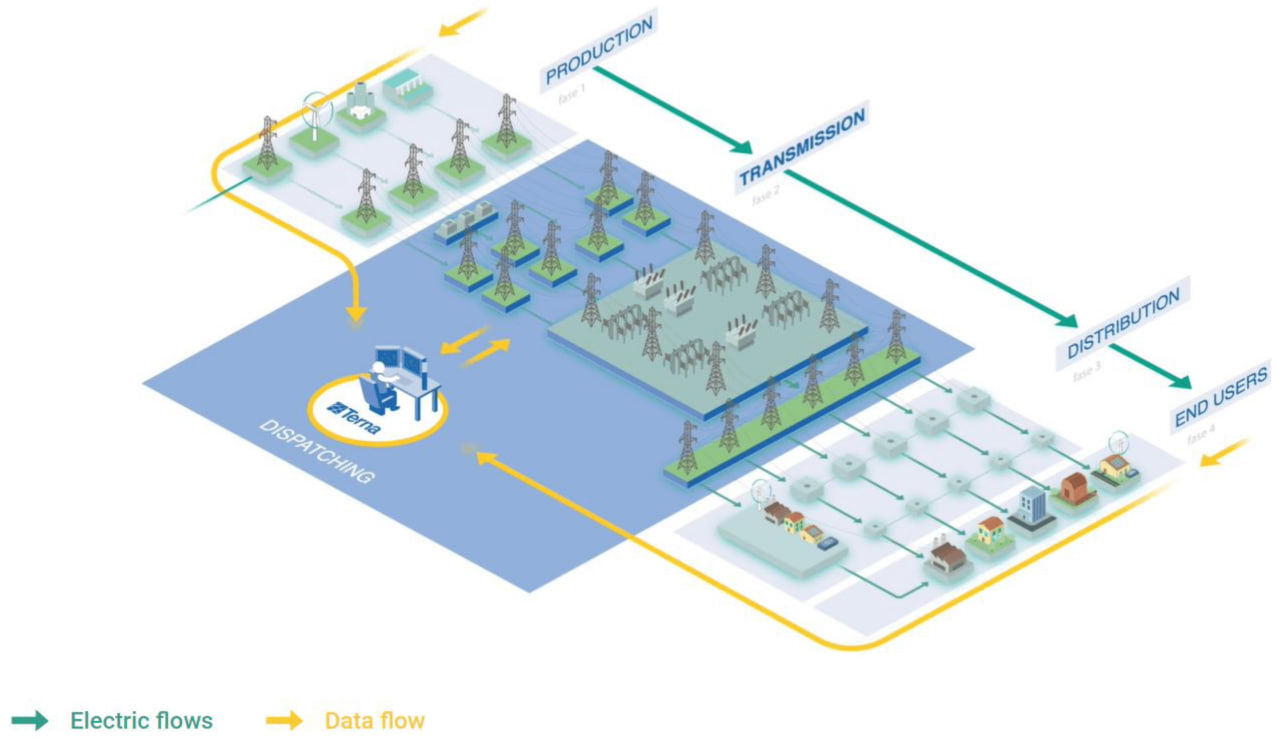
\includegraphics[width=0.8\textwidth]{photo_2023-09-26_14-27-16.jpg}

%         \label{fig:enter-label}
%     \end{figure}
% \end{frame}



\begin{frame}{Stochastic Capacity Expansion Problem (CEP)}

  We formulate the Stochastic Capacity Expansion Problem as a two-stage stochastic program. \pause
  \begin{align*}
    \min_{x} \; & c'x + \bE_{\omega}\left[\cV(x,\omega)\right] \\  \tag{CEP}
    s.t. \;     & 0 \leq x_{n,g} \leq X_{n,g}
  \end{align*}
  \begin{itemize}
    \pause
    \item The first stage determines the capacity expansion \(x_{n,g}\) for each generator \(g \in \cG \) \pause
    \item The second stage solves the Economic Dispatch (ED). \pause
  \end{itemize}

  Where \(\cV(x,\omega)\) is the solution to (ED) in function of the expanded capacities \(x\) and the scenario \(\omega\).
\end{frame}


\begin{frame}{Economic Dispatch (ED) model \; \only<2>{\textcolor{red}{Scary Slide}}}
  \pause \pause
  For a fixed scenarios \(\omega = (\mathcal{PV}, \mathcal{W}, \mathcal{D})\) comprising of respectively solar power, wind power and loads,  \pause
  let \: \( y_{\omega} = (p_{\omega},f_{\omega},ls_{\omega}, s)'\) be the vector containing the power generation, power flows, line shedding and spillage variables. \pause
  \begin{align}
    \min_{y} \; & q'y_{\omega}                                                                                                                                            \\
    s.t. \;     & p_{n,g,t,{\omega}} + bd_{n,t,{\omega}} + \sum_{l \in \cL(n)}f_{n,l,t,{\omega}} + ls_{n,t,{\omega}} + \mathcal{PV}_{n,t,{\omega}} + \cW_{n,t,{\omega}} = \\
                & \quad \quad =  \cD_{n,t,{\omega}} + s_{nt.{\omega}} + bc_{n,t,{\omega}} \nonumber                                                                      \\
                & v_{n,t,{\omega}} = v_{n,t-1,{\omega}} + BCE \cdot bc_{n,t,{\omega}} - BDE \cdot bd_{n,t,{\omega}} + A_{n,t,{\omega}}                                    \\
                & (v_{n,t,{\omega}}, bc_{n,t,{\omega}}, bd_{n,t,{\omega}}) \leq (BV, BC, BD)                                                                              \\
                & p_{n,g,t,{\omega}} \leq p^{\text{max}}_{n,g} + x_{n,g}                                                                                                  \\
                & L^{\text{min}}_{n, l} \leq f_{n,l,t,{\omega}} \leq L^{\text{max}}_{n, l}
  \end{align}

  Where \(v_{n,t,w}\) is the power stored at bus \(n\) at time \(t\).
\end{frame}



\section{Models and sub-Models}


\begin{frame}{Model relaxation description: Intermediate Economic Dispatches (ED-k)}
  \begin{itemize}
    \item We divide the time horizon into \(K\) intervals, \(\{t_{0} = 0 \coloneqq 1,\ldots, t_{1}\},\{t_1+1,\ldots,t_2\},\) \\ \( \ldots,\{t_{K-1}+1,\ldots,t_K \coloneqq T\}\) \pause
    \item We fix a priori the intermediate storage values \(v_{t_k}\) for \(k = 1,\ldots,K\). \pause
    \item We refer to the (ED) problems restricted to each time interval with fixed initial and final storage values as \textbf{(ED-k)} and to its optimal values as and with optimal value \(\mathbf{\cV_{k}(x,v_{t_{k}},v_{t_{k+1},\omega})}\) \pause %this is kind of as saying to the grid, hey you start this storage levels, but must end at this other storage levels
  \end{itemize}

  \begin{oss}
    \begin{equation}\label{Divided ED eq}
      \cV(x,\omega) = \min_{\{v_{t_k}\}_{k=1}^K}\sum_{k=0}^{K-1}\cV_{k}(x,v_{t_{k}},v_{t_k+1},\omega)
    \end{equation}
  \end{oss}

\end{frame}

\begin{frame}{Model relaxation description: Lower Approximation of (ED)}
  Since each function \(\cV_k\) is piecewise linear convex in \(x,v_{t_K},v_{t_{K+1}}\), it can be approximated by a collection of supporting hyperplanes \(\{\pi^w_{i,k}(x,v_{t_k},v_{t_{k+1}})\}\) of each \(\cV_k\). \\ \pause
  An approximation of (ED) is given by: \pause
  \begin{align*}
    \hat{\mathcal{V}}(x,\omega) & = \min_{\{v_{t_k}\}_{k=1}^K} \sum_{k=0}^K \hat{\mathcal{V}}_k(x,v_{t_k},v_{t_{k+1}}) =                           \\
                                & = \min_{\{v_{t_k}\}_{k=1}^K} \sum_{k=0}^K \theta_{k}^{\omega} \tag{ISP}                                          \\
                                & \quad \quad \text{s.t.} \quad \theta_k^{\omega} \geq \pi_{i,k}^{\omega}(x,v_{t_k},v_{t_{k+1}}) \quad \forall i,k
  \end{align*}
  We refer to this problem as the \textbf{Intermediate Storage Problem (ISP)} \pause
  \\ (I know, very original)

\end{frame}
\begin{frame}{Model description: Relaxed Capacity Expansion(CEP-R)}
  %Thus by substituting \(\cV\) with \( \hat{\cV} \) in (CEP) we obtain the following relaxation:
  \begin{align*}
    \label{CEP-A}
    \min_{x} \; & c'x + \bE_{\omega}\left[\cV(x,\omega)\right] \\  \tag{CEP}
    s.t. \;     & 0 \leq x_{n,g} \leq X_{n,g}
  \end{align*}
  \pause
  \begin{align*}
    \label{CEP-R}
    \min_{x} \; & c'x + \bE_w\left[\hat{\cV}(x,w)\right] \\  \tag{CEP-R}
    s.t. \;     & 0 \leq x_{n,g} \leq X_{n,g}
  \end{align*}
  \pause
  Since calculating \( \hat{\cV} \) is straightforward, solving (CEP-R) can be done efficiently with L-shaped or subgradient schemes.
\end{frame}

\section{Decomposition Algorithm}

\begin{frame}{Algorithm}
  % https://q.uiver.app/#q=WzAsMTAsWzEsMCwiXFx0ZXh0e0lucHV0fSJdLFsxLDEsIlxcdGV4dHtSLUNFUH0iXSxbMSwyLCJJU1AoXFxvbWVnYSkgXFw7IFxcZm9yYWxsIFxcb21lZ2FcXGluXFxPbWVnYSJdLFswLDMsIlxcdGV4dHtFRC0xfSJdLFsxLDMsIlxcdGV4dHtFRC0yfSJdLFsyLDMsIlxcZG90cyJdLFszLDMsIlxcdGV4dHtFRC1LfSJdLFsxLDQsIlxcdGV4dHtDb21wdXRlIG5ldyBjdXRzIGZvciB9IFZfayBcXDsgXFxmb3JhbGwgayJdLFs0LDQsIlxcYnVsbGV0Il0sWzEsNSwiXFxoYXR7eF5pfSBcXHRleHR7IGlzIENFUC1vcHRpbWFsfSJdLFswLDFdLFsxLDIsIlxcaGF0e3h9XmkiXSxbMiwzLCJ2X3t0XzB9LHZfe3RfMX0iLDFdLFsyLDQsInZfe3RfMX0sdl97dF8yfSIsMV0sWzIsNV0sWzIsNiwidl97dF97ay0xfX0sdl97dF9rfSIsMV0sWzMsN10sWzQsNywiXFx0ZXh0e0R1YWwgbXVsdGlwbGllcnN9IiwxXSxbNSw3XSxbNiw3XSxbNyw4LCJcXHRleHR7aWYgbmV3IGN1dHN9IiwxXSxbOCwxLCJcXHRleHR7QWRkIGN1dHN9IiwxLHsiY3VydmUiOjV9XSxbNyw5XV0=
  \[\begin{tikzcd}[ampersand replacement=\&]
    \& {\text{Input}} \\
    \& {\text{R-CEP}} \\
    \& {ISP(\omega) \; \forall \omega\in\Omega} \\
    {\text{ED-1}} \& {\text{ED-2}} \& \dots \& {\text{ED-K}} \\
    \& {\text{Compute new cuts for } V_k \; \forall k} \&\&\& \bullet \\
    \& {\hat{x^i} \text{ is CEP-optimal}}
    \arrow[from=1-2, to=2-2]
    \arrow["{\hat{x}^i}", from=2-2, to=3-2]
    \arrow["{v_{t_0},v_{t_1}}"{description}, from=3-2, to=4-1]
    \arrow["{v_{t_1},v_{t_2}}"{description}, from=3-2, to=4-2]
    \arrow[from=3-2, to=4-3]
    \arrow["{v_{t_{k-1}},v_{t_k}}"{description}, from=3-2, to=4-4]
    \arrow[from=4-1, to=5-2]
    \arrow["{\text{Dual multipliers}}"{description}, from=4-2, to=5-2]
    \arrow[from=4-3, to=5-2]
    \arrow[from=4-4, to=5-2]
    \arrow["{\text{if new cuts}}"{description}, from=5-2, to=5-5]
    \arrow["{\text{Add cuts}}"{description}, curve={height=40pt}, from=5-5, to=2-2]
    \arrow[from=5-2, to=6-2]
  \end{tikzcd}\]
\end{frame}

% \begin{frame}{Algorithm}
%   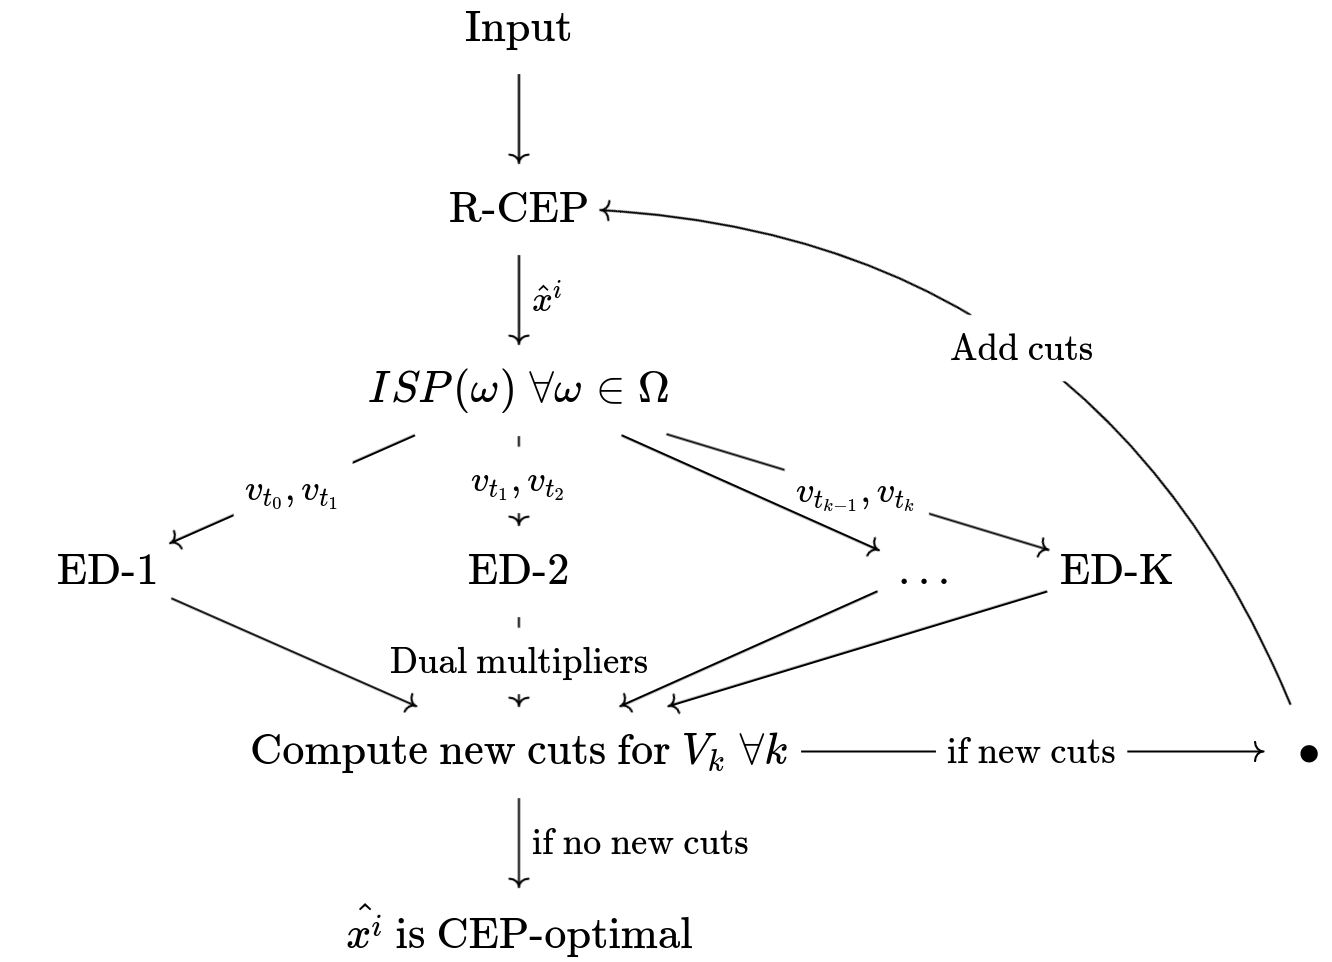
\includegraphics[width = 0.7\linewidth]{Alg.png}
% \end{frame}
% \begin{frame}{Algorithm description} %maybe we can devide this description in the previous slides
%   INPUT: Provide a lower bound for \(\theta_k^{\omega}\) for \(k=1,\ldots,K\) and \( \omega \in \Omega \) and a trial action \(\hat x^0\)
%   \pause
%   \begin{enumerate}[label = {\arabic*}]
%     \item Warm-Start: Calculate initial approximation for \(\mathcal{V}\) for all \(\omega \in \Omega\) around \(\hat{x}^0\). \pause
%     \item For \(i = 1,\ldots,N\): \pause
%           \begin{enumerate}[label = {2.\arabic*}]
%             \item Solve current relaxation (CEP-R) and obtain new trial action \(\hat x^i\). \pause
%             \item For \(\omega \in \Omega \) (in parallel): \pause
%                   \begin{enumerate}[label = {2.1.\arabic*}]
%                     \item Solve the (ISP) approximation problem \(\hat{\mathcal{\cV}}(\hat{x}^{(i)},\omega)\) and obtain intermediate storage values \(\hat{v}^i_k\) for \(k=1,\ldots,K\).\pause
%                     \item Solve (ED-k) (in parallel) for each time step.\pause
%                     \item Using dual multipliers, compute a supporting hyperplane for \(\cV_k\) around \(\hat{x}^i, \hat{v}^i_k, \hat{v}^i_{k+1}\) for \(k=0,\ldots,K-1\).\pause
%                     \item Add the supporting hyperplanes to the approximation problems (ISP) and(CEP-R) \(\hat{\mathcal{V}}(\hat{x}^{(i)},\omega)\).
%                   \end{enumerate}
%           \end{enumerate}
%   \end{enumerate}
% \end{frame}

% \begin{frame}{Algorithm description}
%   INPUT: Provide a lower bound for \(\theta_k^{\omega}\) for \(k=1,\ldots,K\) and \( \omega \in \Omega \) and a trial action \(\hat x^0\)

%   \begin{tabular}{@{}p{0.95\textwidth}}
%     1. Warm-Start: Calculate initial approximation for \(\mathcal{V}\) for all \(w \in \Omega\) around \(\hat{x}^0\). \\
%     2. For \(i = 1,\ldots,N\): \\
%     \quad 2.1. For \(w \in \Omega \) (in parallel): \\
%     \quad\quad\quad 2.1.1. Solve the (ED) approximation problem \(\hat{\mathcal{V}}(\hat{x}^{(i)},\omega)\) and obtain 
%     \\ \quad\quad\quad\quad  intermediate storage values \(\hat{v}^i_k\) for \( k=1,\ldots,K\). \\
%     \quad\quad\quad 2.1.2. Solve (ED) (in parallel) for each time step \(k = 0,\ldots,K-1\),
%     \\ \quad\quad\quad\quad\(V_k(\hat{x}^i,\hat{v}^i_k, \hat{v}^i_{k+1},\omega)\). \\
%     \quad\quad\quad 2.1.3. Using dual multipliers, compute a supporting hyperplane for \(V_k\) around 
%     \\ \quad\quad\quad\quad\(\hat{x}^i, \hat{v}^i_k, \hat{v}^i_{k+1}\) for \(k=0,\ldots,K-1\). \\
%     \quad\quad\quad 2.1.4. Add the supporting hyperplanes to the approximation problem (CEPR)
%     \\ \quad\quad\quad\quad  \(\hat{\mathcal{V}}(\hat{x}^{(i)},\omega)\). \\

%   \end{tabular}
% \end{frame}


\section{Convergence results}
\begin{frame}{Convergence results 2}
  \begin{itemize}
    \item Since \((CEP-R) \leq (CEP)\) if a \((CEP-R)\) optimal solution has the same cost for \((CEP)\) then it's also \((CEP)\)-optimal. \pause
  \end{itemize}

  \hfill \\


  \textbf{Remark 1:} It is sufficient to prove that after a finite number of steps \((i)\) of the algorithm we have:
  \begin{equation}
    \hat{\cV}(\hat x^i,\omega) = \cV(\hat x^i,\omega)  \text{ for all }  \omega \in \Omega
  \end{equation}


\end{frame}


\begin{frame}{Convergence results 3}
  \begin{oss}
    After a finite number of iterations no new cuts are found for \(\cV_k\).
  \end{oss}
  \begin{proof}
    \begin{align}
       & \uncover<2->{\#\{p \mid p \text{ is a normal vector of a supporting hyperplane of } \mathcal{V}_k\} \leq \nonumber }\uncover<3->{ \\
       & \#\{\text{dual solutions } p=q'B^{-1} \text{ of (ED-k) for varying } x, v_{t_k}, v_{t_{k+1}}\} \leq \nonumber }\uncover<4->{      \\
       & \#\{\text{basis matrices of (ED-k)}\} < \infty }
    \end{align}
    \pause \pause \pause \pause
    After a finite number of steps: \pause
    \begin{itemize}

      \item new cut: \(\bar c (x,v)= \textcolor{deepblue}{p}'(x,v) + b\)  \pause
      \item an old cut: \(\pi(x,v) = \textcolor{deepblue}{p}'(x,v) + \bar b\)

    \end{itemize}


  \end{proof}
\end{frame}


\begin{frame}[noframenumbering]{Convergence results 3}



  \begin{tikzpicture}[scale=1]
    % Draw axes
    \draw[->] (-1,0) -- (4,0) node[right] {$x$};
    \draw[->] (0,-1) -- (0,3) node[above] {$y$};

    % Define function breakpoints
    \def\xbreak{2}
    \def\ybreak{2}

    % Draw piecewise function
    \draw[thick] (0,2.3) -- (\xbreak,\ybreak);
    \draw[thick] (\xbreak,\ybreak) --  (4,3);

    % Draw tangent line (touching the curve at one point)
    \draw[thick, red] (0,1.5) -- (4,2.5);

    % Mark the touching point
    \filldraw[black] (\xbreak,\ybreak) circle (1pt);

    % Draw parallel line slightly beneath the first one
    \draw[thick, green] (0,1) -- (4,2);

    \draw (3,3) node {$\cV_k$};
    \draw (1,1.90) node[red] {$\pi$};
    \draw (1,1.41) node[green] {$\bar c$};

  \end{tikzpicture}
  \pause
  \\ Since both are supporting hyperplanes it follows that \( b = \bar b\) \\(and therefore \( \bar c\) is not a new cut).
\end{frame}
\begin{frame}{Convergence results 4}
  \begin{oss}
    If after the \(i\)-iteration no new cuts are added for some \(i\) and \(k\) then \(\hat{\cV}_k(\hat x^i, \hat v_{k},\hat v_{k+1}) = \cV_k(\hat x^i, \hat v_{k},\hat v_{k+1}). \) \\ \pause
    Where \( \hat{\cV}_k(\hat x^i,\hat v_{t_k},\hat v_{t_{k+1}},{\omega}) = \max_i \pi_{i,k}^{\omega}(\hat x^i,\hat v_{t_k},\hat v_{t_{k+1}})\) be the current supporting hyperplane approximation of \(\cV_k\).
    \pause
  \end{oss}
  \begin{proof}

    Let \(\bar c_k^{\omega}(x,v_{t_k}) \coloneqq p'(x-\hat x^i, v_{t_k}-\hat v_{t_k}) + V_k(\hat x^i,\hat v_{t_k})\) be the new cut found after the \(i\)-th iteration. \\ \pause
    Since \(\bar c\) is not a new cut we have \( \bar c(\hat x^i,v_{t_k}) \leq \hat{\cV_k}(\hat x^i,v_{t_k})\). \pause
    We have thus \[\cV_k(\hat x^i,\hat v_{t_k}) \geq \hat \cV_k(\hat x^i,\hat v_{t_k}) \geq \bar c (\hat x^i,\hat v_{t_k}) = \cV_k(\hat x^i,\hat v_{t_k})\] \pause which concludes the proof.
  \end{proof}

\end{frame}

\begin{frame}{Convergence results 5}
  In conclusion, we have \(\hat{\cV}_k(\hat x^i, v_{t_k},v_{t_{k+1}},\omega) = \cV_k(\hat x^i, v_{t_k},v_{t_{k+1}},\omega)\) for all \(\omega,k\). \pause \\
  Thus \( \hat \cV(\hat x^i,\omega) = \cV(\hat x^i,\omega) \). \pause
  \hfill \\
  \hfill \\
  \begin{prop}
    The algorithm converges after a finite number of iterations and \(\hat x^i\) is an optimal solution for (CEP).
  \end{prop}
\end{frame}

\begin{frame}{Future implementation in Pypsa}
  \begin{itemize}
    \item We are currently implementing this and other stochastic methods within the Pypsa \cite{PyPSA} framework using the Linopy \cite{Hofmann2023} modeling package in Python. \pause
    \item We expect improved convergence speed respect to the L-shaped method, especially when leveraging parallel processing capabilities.
  \end{itemize}

  \vspace{1cm}

\end{frame}
\begin{frame}{Conclusions and future perspectives.}
  \begin{itemize}
    \item The specific structure of the intertemporal constraints makes it possible do develop tailored optimization algorithms for (CEP). \pause
    \item The presented method can be also applied to other linear models such as DC-OPF. \pause
    \item Care must be taken for intra-temporal constraints such as ramp up or ramp down constraints. \pause
    \item Develop heuristics for the choice of the number of time intervals \(K\). \pause
    \item Examine generalizations to multistage stochastic programs. \pause
  \end{itemize}

\end{frame}

\begin{frame}
  \vfill
  Thank you for your attention.

  \vfill
  \vfill
  \vfill
  \begin{footnotesize}
    gabor.riccardi01@universitadipavia.it \\
    \url{https://www.compopt.it}
  \end{footnotesize}
\end{frame}
\section{Bibliography}
\appendix
\begin{frame}{}
  Some references:\\[2em]
  \begin{footnotesize}
    \printbibliography[
      %heading=bibintoc,
      title={Bibliography}]
  \end{footnotesize}
\end{frame}

% \begin{frame}[noframenumbering]{Literature}
%   \begin{itemize}
%     \item Traditional stochastic capacity expansion methods, such as the L-shaped method, may perform poorly as the number of expansion possibilities increases.
%    
% \end{frame}


\begin{frame}[noframenumbering]{Adequacy Assessment of the Electrical Grid}
  \begin{itemize}
    \item Measuring the ability of the electric power system to react to adverse uncertain condition has become increasingly importan.
    \item Member States wishing to introduce capacity mechanisms can do so if an adequacy concern is identified in the ERAA study, a pan-European adequacy assessment for up to 10 years ahead.
    \item Due to the scale of the ERAA study, ERAA 2022 considered a reduced stochastic problem with three scenarios.
    \item In \cite{DecompAlg}, Daniel A'vila introduced a decomposition algorithm based on subgradient approximations was introduced

  \end{itemize}
\end{frame}

\begin{frame}[noframenumbering]{Power Grid Optimization}
  \begin{itemize}
    \item Optimal Power Flow (OPF) \hfill \textcolor{gray}{\cite{MathProgForm}}
          \begin{itemize}
            \item AC OPF: exact physical model
            \item Security-Constrained OPF (SCOPF) -- Includes contingencies to guarantee system security under failures.
            \item DC OPF and other linearized models \hfill \textcolor{gray}{\cite{LinRelBien} }
            \item other relaxations.
          \end{itemize}

    \item Unit Commitment -- Determines on/off status of power units, ignoring grid constraints.
    \item Economic Dispatch (ED) -- Minimizes generation cost, ignoring grid constraints.
  \end{itemize}
  % Blue arrow on the side of the text
  \begin{tikzpicture}[overlay, remember picture]
    \node at ([shift={(0.9,-1)}]current page.north west) (end0) {}; % Adjust for positioning
    \node at ([shift={(0.9,3)}]current page.south west) (start0) {}; % Adjust for positioning
    \draw[->, thick, blue] (start0) -- (end0) node[midway, fill=white, rotate=90] {Time / Exactness};

    \node at ([shift={(0.3,-1)}]current page.north west) (start1) {}; % Corrected position and syntax
    \node at ([shift={(0.3,3)}]current page.south west) (end1) {}; % Corrected position and syntax
    \draw[->, thick, yellow] (start1) -- (end1) node[midway, fill=white, rotate=90] {Stochasticity}; % Corrected spelling and syntax
  \end{tikzpicture}

  \vfill
  \textbf{Capacity expansion problem:} Based on Economic Dispatch models with added flow balance at bus nodes and various scenarios.
\end{frame}


%possible questions:
% 1) what is the relation between cep-a and the adequacy Assessment?
% Adequacy Assessment span multiple years, over which a certain capability of expanding the grid is expected.
% But the is also ma maximum expected capability to expand thegrid.
% 2) Comparison with L-shaped algorithm (i am a potato)



\end{document}








